\documentclass{article}
\usepackage{setspace}
\usepackage[text={6.5in,8.5in},centering]{geometry}
\geometry{verbose,a4paper,tmargin=2.4cm,bmargin=2.4cm,lmargin=2.4cm,rmargin=2.4cm}
\usepackage{graphicx,amsmath,cases,multirow,appendix,graphicx,xcolor}

\setlength\parindent{0pt}

\newcommand{\note}[1]{\colorbox{gray!30}{#1}}
\newcommand{\ind}{\-\hspace{1cm}}

\begin{document}

\noindent\makebox[\textwidth][c]{\Large\bfseries Lecture 9 -- 1-D Stability Analysis - Part 2}
\rule[0.5ex]{\linewidth}{1pt}
\textbf{Today:} 1D stability cont., non-dimensionalization, and paper discussion\\
\textbf{Next class:} 2 sp. LV competition (Bring laptops -- \emph{might} need them depending on how far we get)\\
\rule[0.5ex]{\linewidth}{1pt}

\textbf{Ricker plots \& Intuitive notion of Lyapunov exponent}
\begin{center}
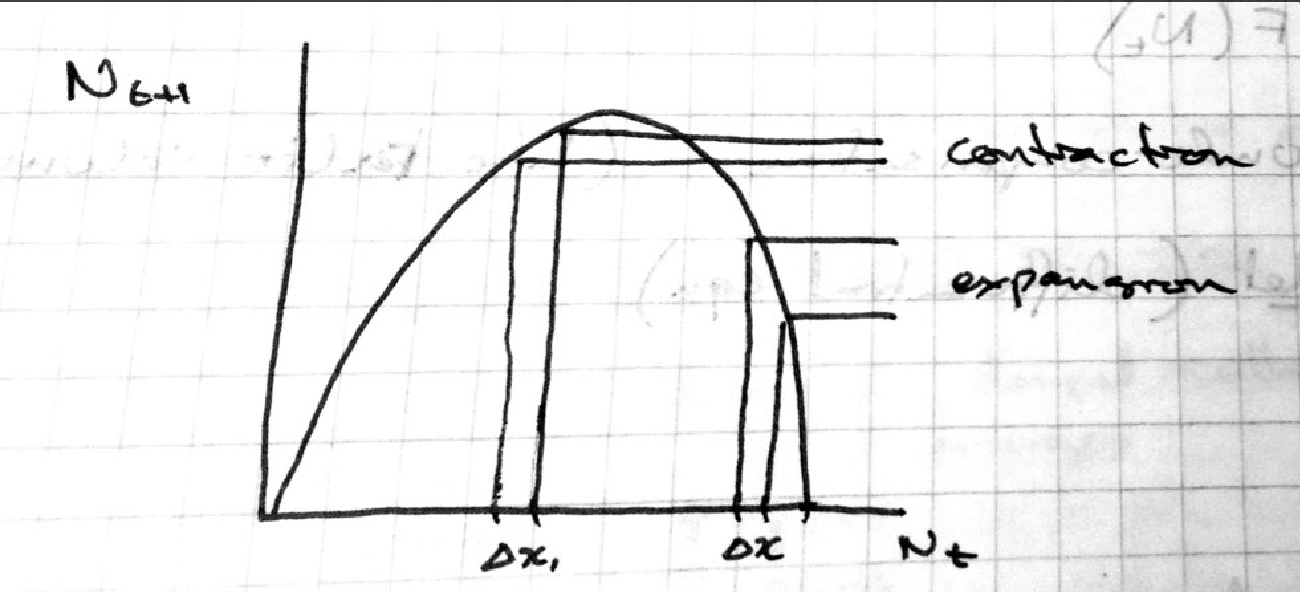
\includegraphics[width=8cm]{figs/RickerLyapunov.pdf}\\
$\to$ The larger $r_d$, the steeper the slopes, the more expansion.
\end{center}

\rule[0.5ex]{\linewidth}{1pt}

\textbf{Local stability analysis}\\
Through simulation we found $r_d<2$ for $N^*=K$ to be stable\\
\ind (either monotonic dampening or damped oscillations).
\begin{center}
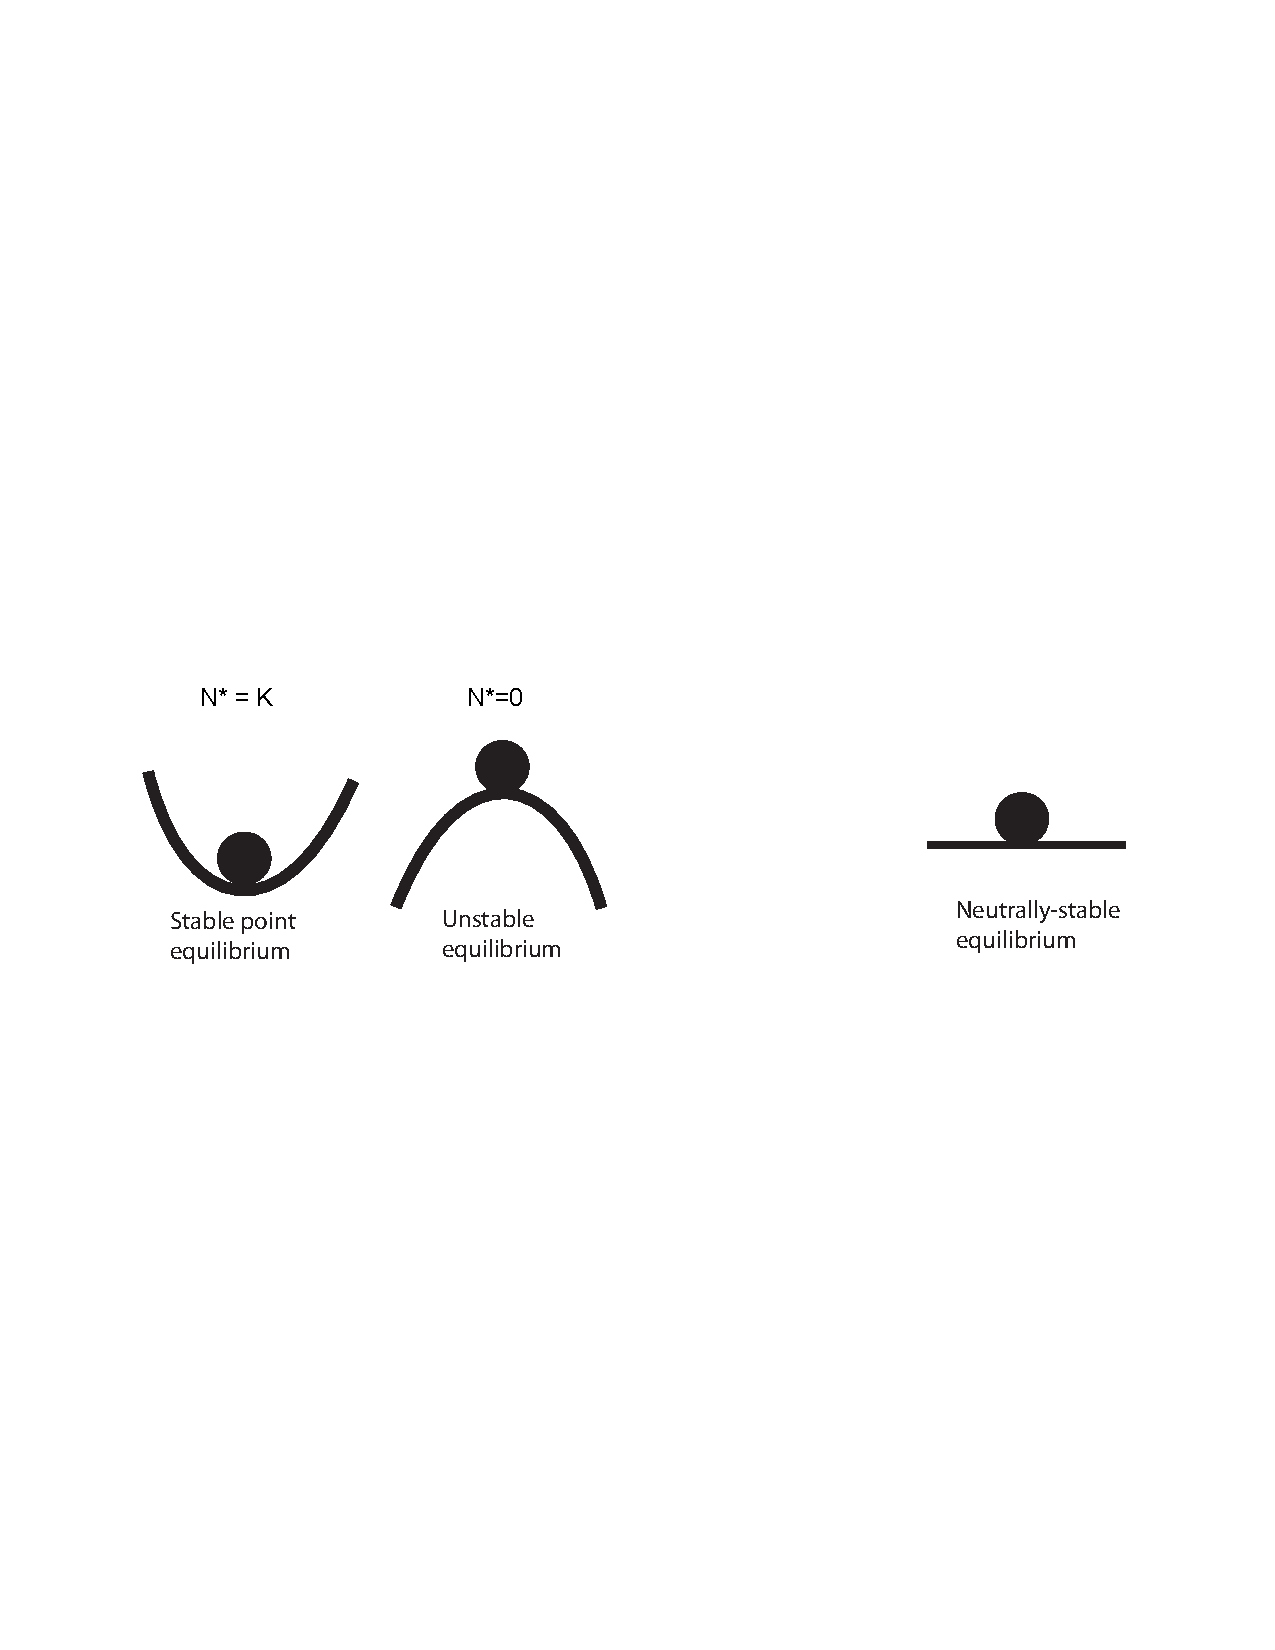
\includegraphics[width=8cm]{figs/ballcup2.pdf}
\end{center}

Now let's determine this formally...

\textbf{Discrete-time model:}
\begin{equation*}
	N_{t+1}= F(N_t)
\end{equation*}
\textbf{Step 1}:  Solve $F(N)$ for $N^*$:
\begin{align*}
	F(N_t)=& N_t+r_d N_t \left( 1-\frac{N_t}{K}\right)\\
	\text{By definition:}\; \; F(N^*)=N_t&\\
	F(N^*)=& N_t=N_t + r_d N_t - \frac{r_d N_t^2}{K}\\
	\text{Solve for} \; N_t: \;\;\;\;0=& r_d N_t-\frac{r_d N_t^2}{K}\\
	\frac{r_d N_t^2}{K}=& r_d N_t\\
	r_d N_t^2 =& r_d N_t K\\
	\to N^* =& K \; \text{and} \; N^*=0\\
\end{align*}
\textbf{Step 2}: Find slope of $F(N_t)$ evaluated at $N^*$:
\begin{equation*}
	F'(N^*)=\left.\frac{d F(N_t)}{dN}\right\vert_{N^*}
\end{equation*}
\begin{center}
$\boxed{\text{If }\vert F'(N^*)\vert <1 \to \text{ stable.}}$
\end{center}
For discrete logistic:
\begin{align*}
	F'(N^*)&=1+ r_d - 2 r_d \frac{N^*}{K}\\
	&= 1+r_d- 2 r_d \frac{K}{K}\\
	&= 1-r_d
\end{align*}
\begin{center}
\textbf{Thus, discrete logistic reaches stable point equilibrium when} $0 < r_d< 2$.
\end{center}

\begin{center}
	\note{Project figure in Keynote}\\
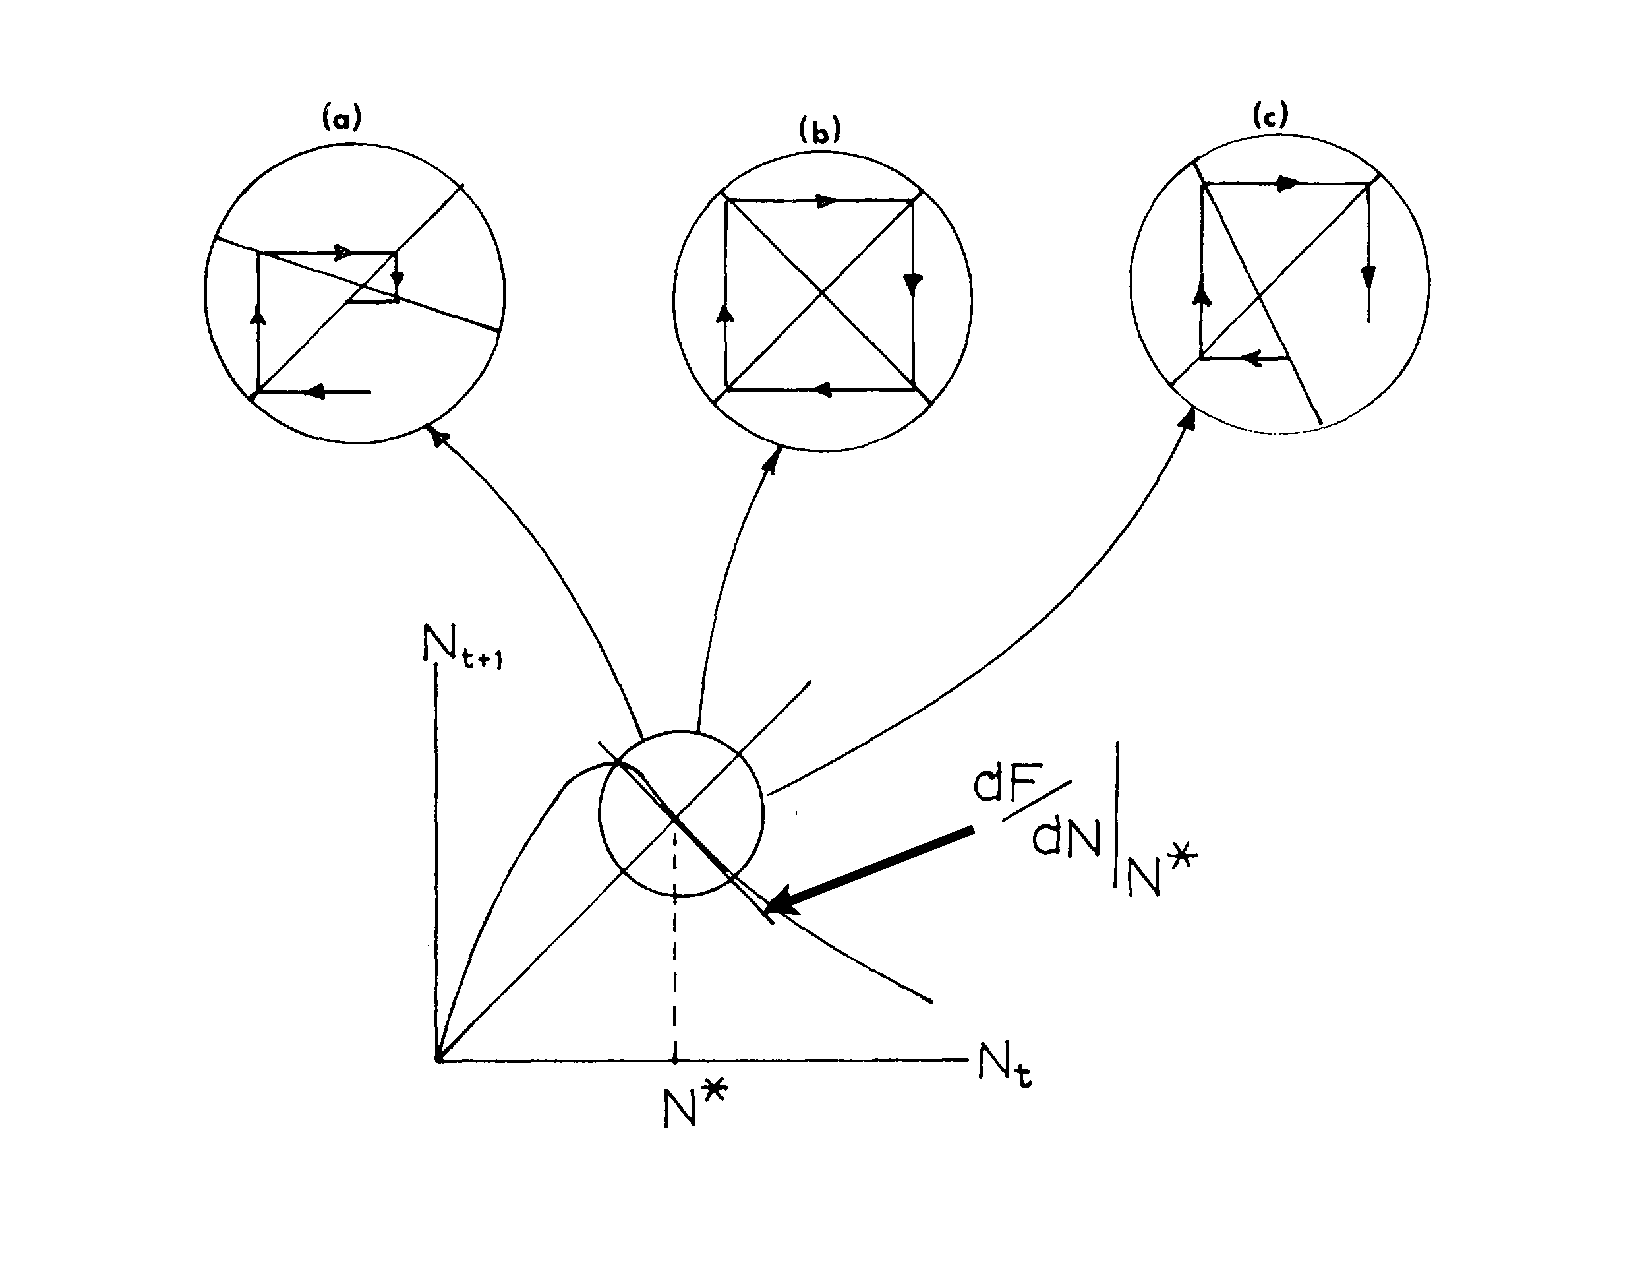
\includegraphics[width=5cm]{figs/RickerSlope.pdf}
\end{center}

\rule[0.5ex]{\linewidth}{1pt}

\textbf{Continuous-time model:}
\begin{equation*}
\frac{dN}{dt}=f(N)=rN\left(1-\frac{N}{K}\right)
\end{equation*}

\textbf{Step 1}:  Solve $f(N)$ for $N^*$:
\begin{align*}
	\text{By definition:  At}\; N^{*} \; \text{when} \; f(N^*)=0&\\
	0 & = rN-\frac{rN^2}{K}\\
	\frac{rN^2}{K}&=rN\\
	rN^2&=rNK\\
	\to N^*& = K \; \text{and} \; N^* =0	
\end{align*}

\textbf{Step 2}:  Find slope of $f(N)$ at $N^*$.  
\begin{equation*}
	f'(N^*)=\left.\frac{d f(N_t)}{dN}\right\vert_{N^*}
\end{equation*}
\begin{center}
	$\boxed{\text{If } f'(N^*) < 0 \to \text{ stable.}}$
\end{center}
\ind \ind For continuous-logistic:\\
\begin{align*}
	f'(N^*=K)&=\frac{d}{dN}\left(rN-\frac{rN^2}{K}\right)\\
	&=r-\frac{2r N}{K}\\
	&= r- \frac{2r K}{K}\\
	&= r-2r\\
	&= -r
\end{align*}

\begin{center}
\textbf{Thus, continuous logistic reaches stable point equilibrium when} $r>0$.
\end{center}

\rule[0.5ex]{\linewidth}{1pt}

\textbf{Summary}\\
Step \#1: Solve for $N^*$.\\
Step \#2: Evaluate $f'(N^*)$\\
\ind \ind For discrete:\\
\ind \ind \ind Stable if $\vert F'(N^*) \vert <1$\\
\ind \ind \ind \ind (for discrete logistic, stable if $0<r_d<2$)\\
\ind \ind For continuous:\\
\ind \ind \ind Stable if $f'(N^*) <0$\\
\ind \ind \ind \ind (for continuous logistic, stable if $r>0$)\\

\rule[0.5ex]{\linewidth}{1pt}

\textbf{ 1-D Stability analysis - Dig deeper}
(In discrete time, but same applies to continuous time models)
\begin{equation*}
	N_{t+1}=F(N_t) \; \; \to \;\; N^*
\end{equation*}
Now add small perturbation to $N^*$ by adding $n$:
\begin{equation*}
	N_t = N^* + n_t
\end{equation*}
We therefore expect:
\begin{equation*}
	N_{t+1} = F(N^* + n_t)
\end{equation*}

We want to know if popn will return to $N^*$, but will ask a slightly different question to get the answer:

\vspace{0.5cm}

Since 
\begin{equation*}
	n_t=N_t-N^*
\end{equation*}
can write
\begin{equation*}
	n_{t+1}=N_{t+1}-N^*
\end{equation*}
Thus:
\begin{equation*}
	n_{t+1} = F(N^* + n_t) - N^*
\end{equation*}

\begin{center}
	\textbf{Thus the question is:  Does $n_t$ grow or shrink with time?}
\end{center}

\begin{center}
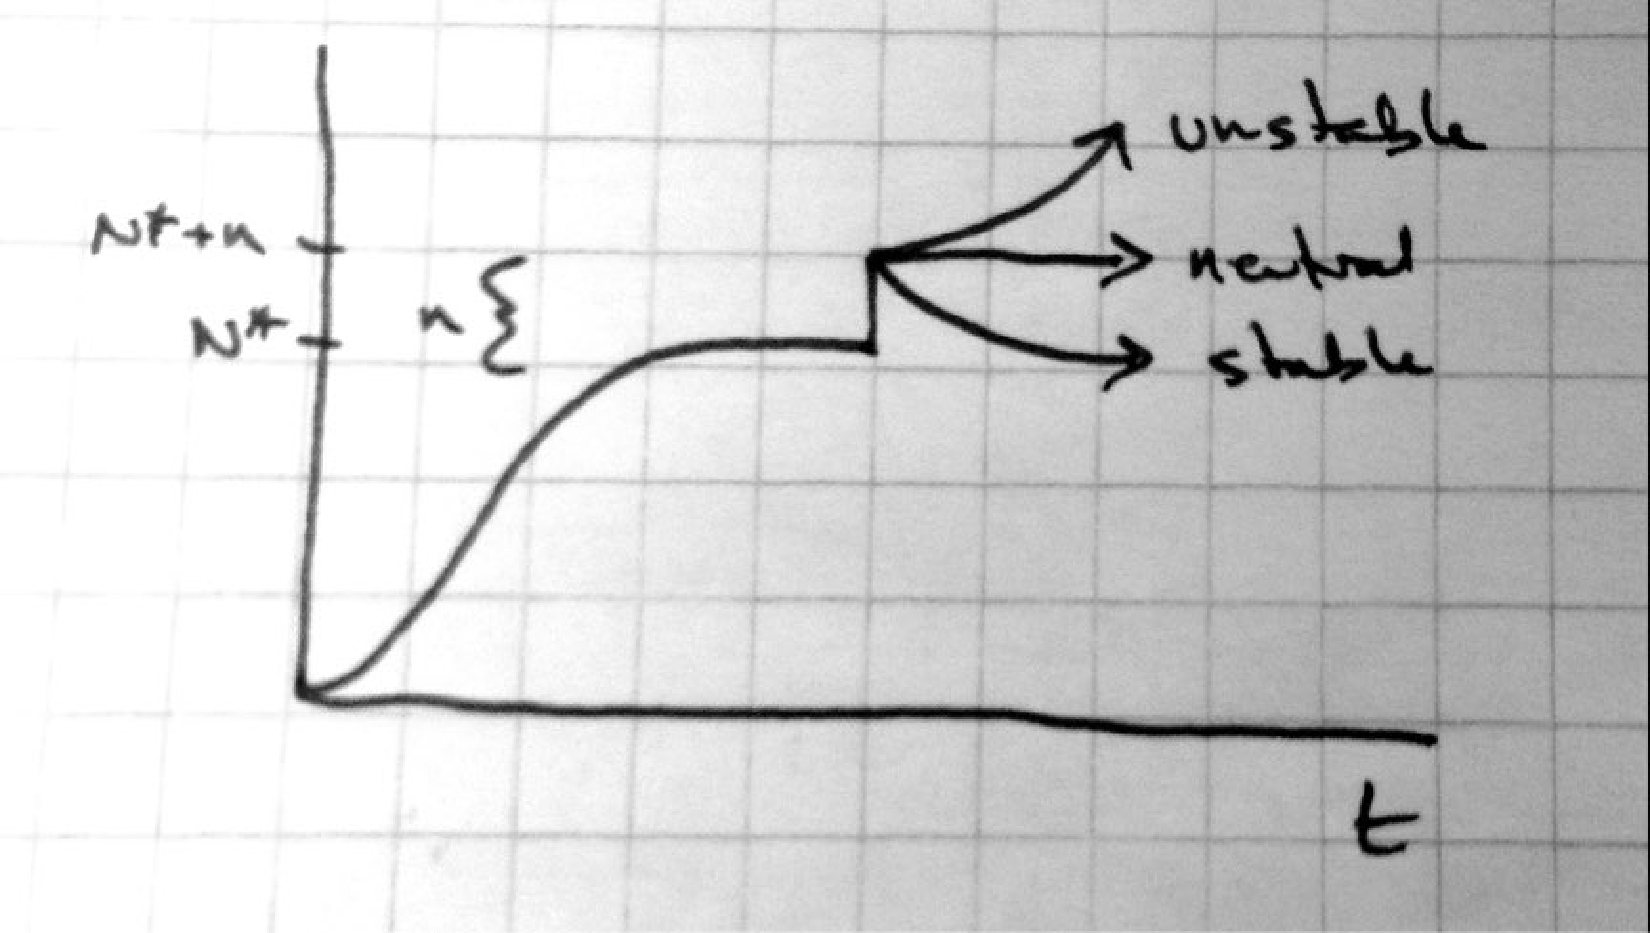
\includegraphics[width=4cm]{figs/Perturb.pdf}
\end{center}

Q: How do we find the solution of $F(N^* + n_t)$?\\
\ind  ($F$ could be a very complicated function!)

A: We approximate it:
\begin{align*}
	\underbrace{F(N^* + n_t)}_y \approx \underbrace{F(N^*)}_{intercept}+ \underbrace{F'(N^*)}_{slope}  \cdot \underbrace{n_t}_x
\end{align*}

\rule[0.5ex]{\linewidth}{1pt}

\textbf{Taylor Series}

Recall polynomial series:
\begin{equation*}
	y=\sum_{i=0}\beta_i x^i
\end{equation*}

Taylor series is similar, but with derivatives...
\begin{equation*}
	F(N^*+n_t)= \sum_{i=0}^\infty \frac{F^{(i)}(N^*)}{i!}n_t^i = F(N^*) + \underbrace{\frac{F'(N^*)}{1!}n_t^1 + \frac{F''(N^*)}{2!} n_t^2 + \frac{F'''(N^*) }{3!}n_t^3 + ...}_{\text{h.o.t.}}
\end{equation*}

\begin{center}
\note{Show figure from \emph{'Class-Ex-TaylorExp.R'}.}
\end{center}

\emph{Higher order terms} get smaller and smaller.\\
First two terms are good approximation when $n_t$ is small.

Thus:
\begin{align*}
	n_{t+1}& =F(N^*+n_t)-N^*\\
	& \approx F(N^*)+F'(N^*) \cdot n_t - N^*\\
	& \approx N^* + F'(N^*) \cdot n_t - N^*\\
	& \approx F'(N^*) \cdot n_t \\
	& = \lambda n_t \quad \quad (\lambda \text{ is the ``eigenvalue'' (for single-spp. model))!}
\end{align*}

\vspace{1cm}

\ind \ind \ind If $\lambda <1 \to n_{t+1} < n_t \to $ Perturbation decays (i.e. stable system)\\
\ind \ind \ind If $\lambda > 1 \to n_{t+1} < n_t \to $ Perturbation expands (i.e. unstable system)\\

Note that $n_t$ could be a \emph{removal} (i.e. $n_t<0$) of individuals (rather than an \emph{addition}).\\

Thus \textbf{for discrete-time model:}\\
\begin{equation*}
\boxed{\vert F'(N^*)\vert < 1 \; \text{ for stability}}
\end{equation*}
\begin{align*}
-1<\lambda &< 0 \to \text{decay w/ damped oscillations}\\
 0<\lambda &< 1 \to \text{geometric decay}\\
 \lambda &> 1 \to \text{geometric growth}\\
 \lambda &<-1 \to \text{divergent oscillations}\\
\end{align*}
\begin{center}
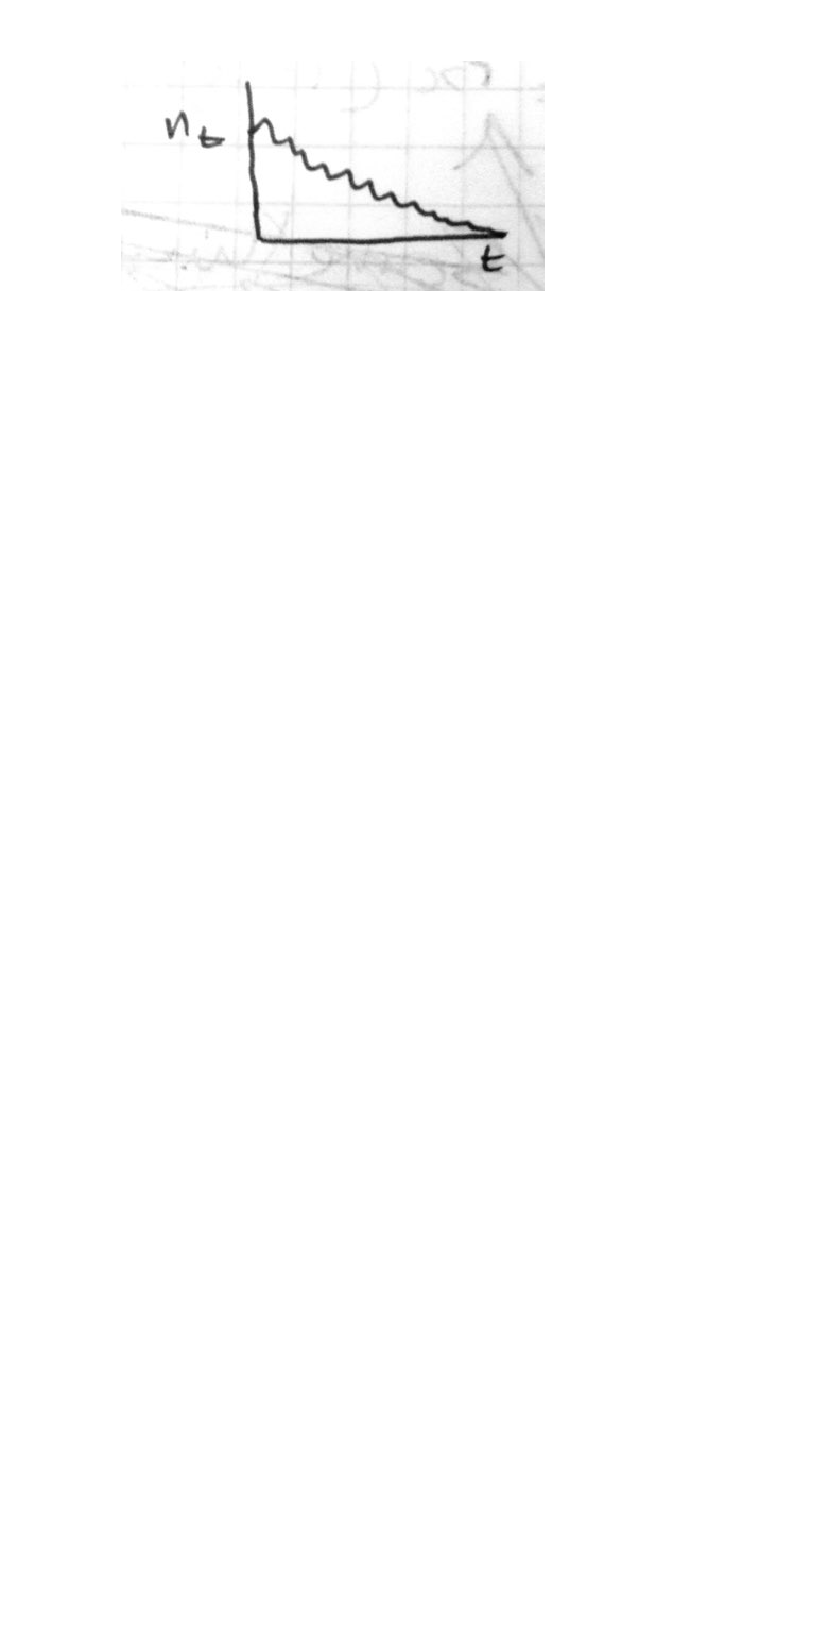
\includegraphics[width=3cm]{figs/DecayOscil.pdf}
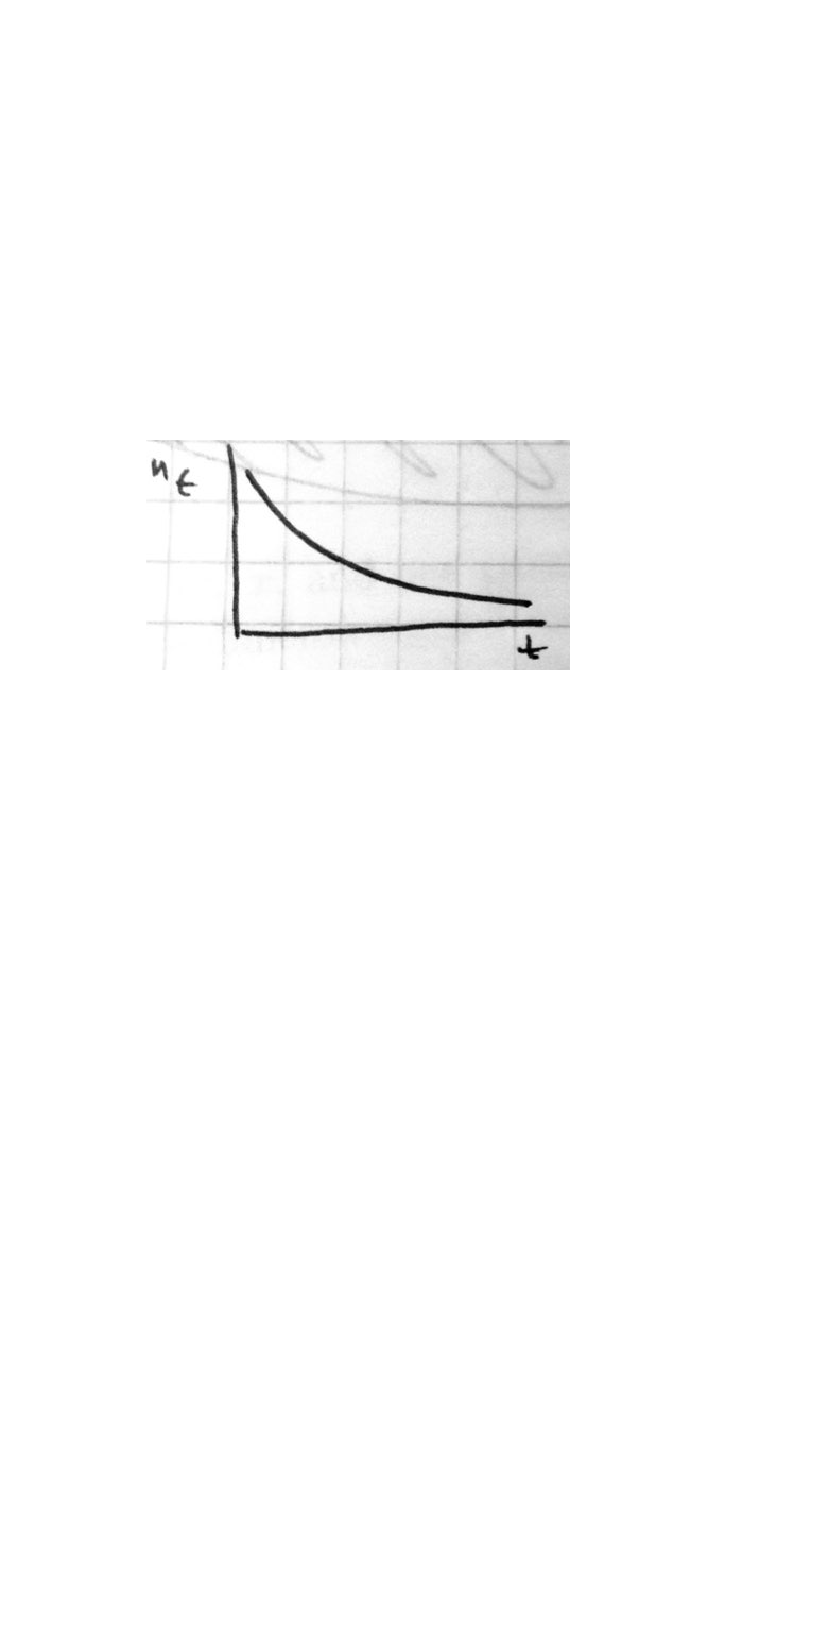
\includegraphics[width=3cm]{figs/Decay.pdf}
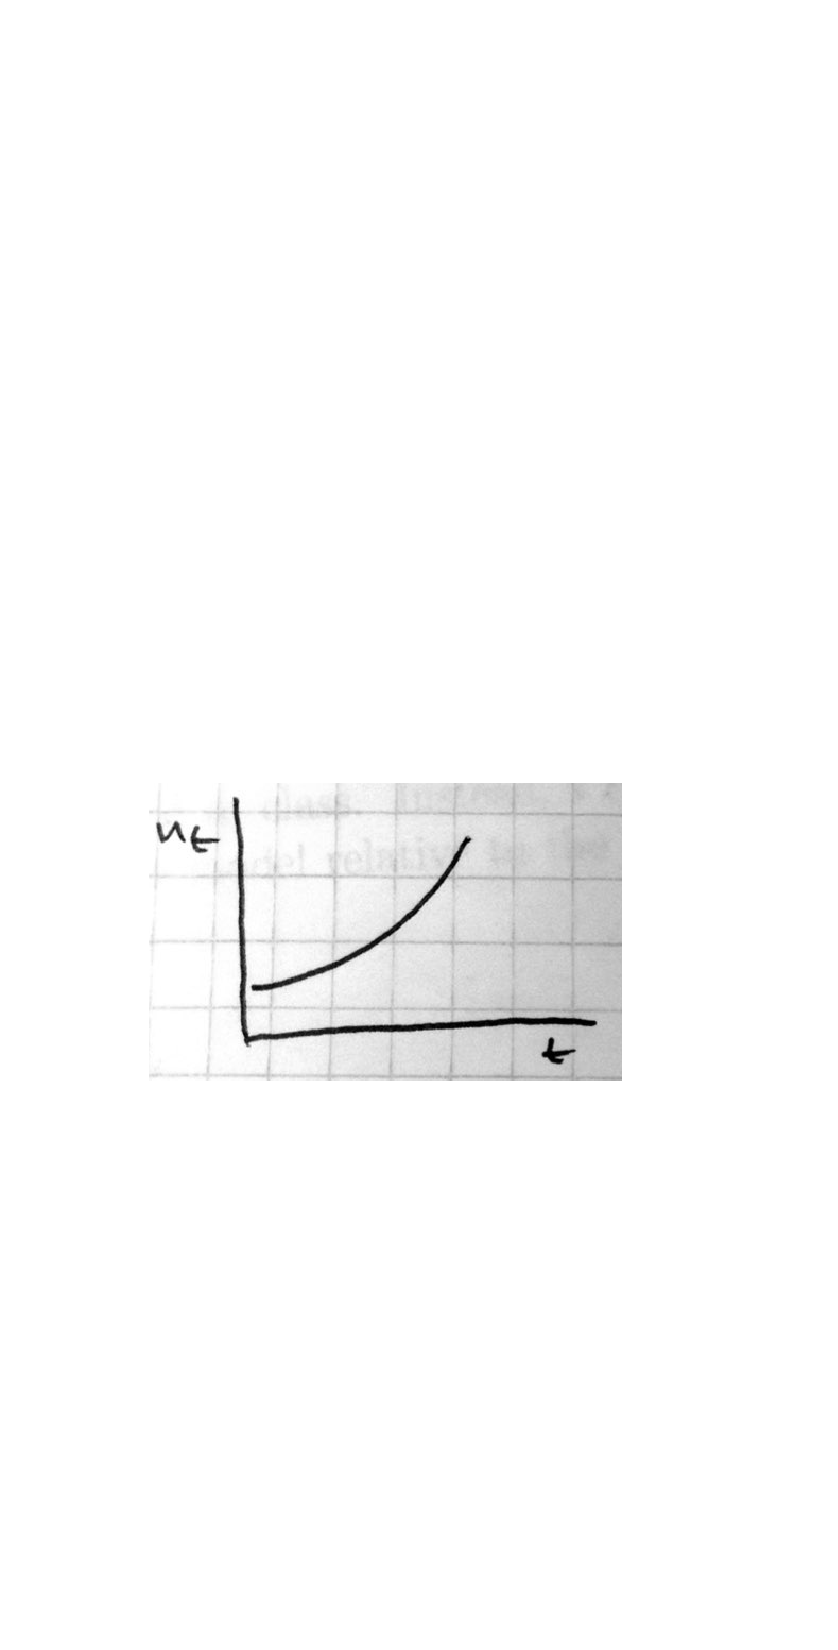
\includegraphics[width=3cm]{figs/Growth.pdf}
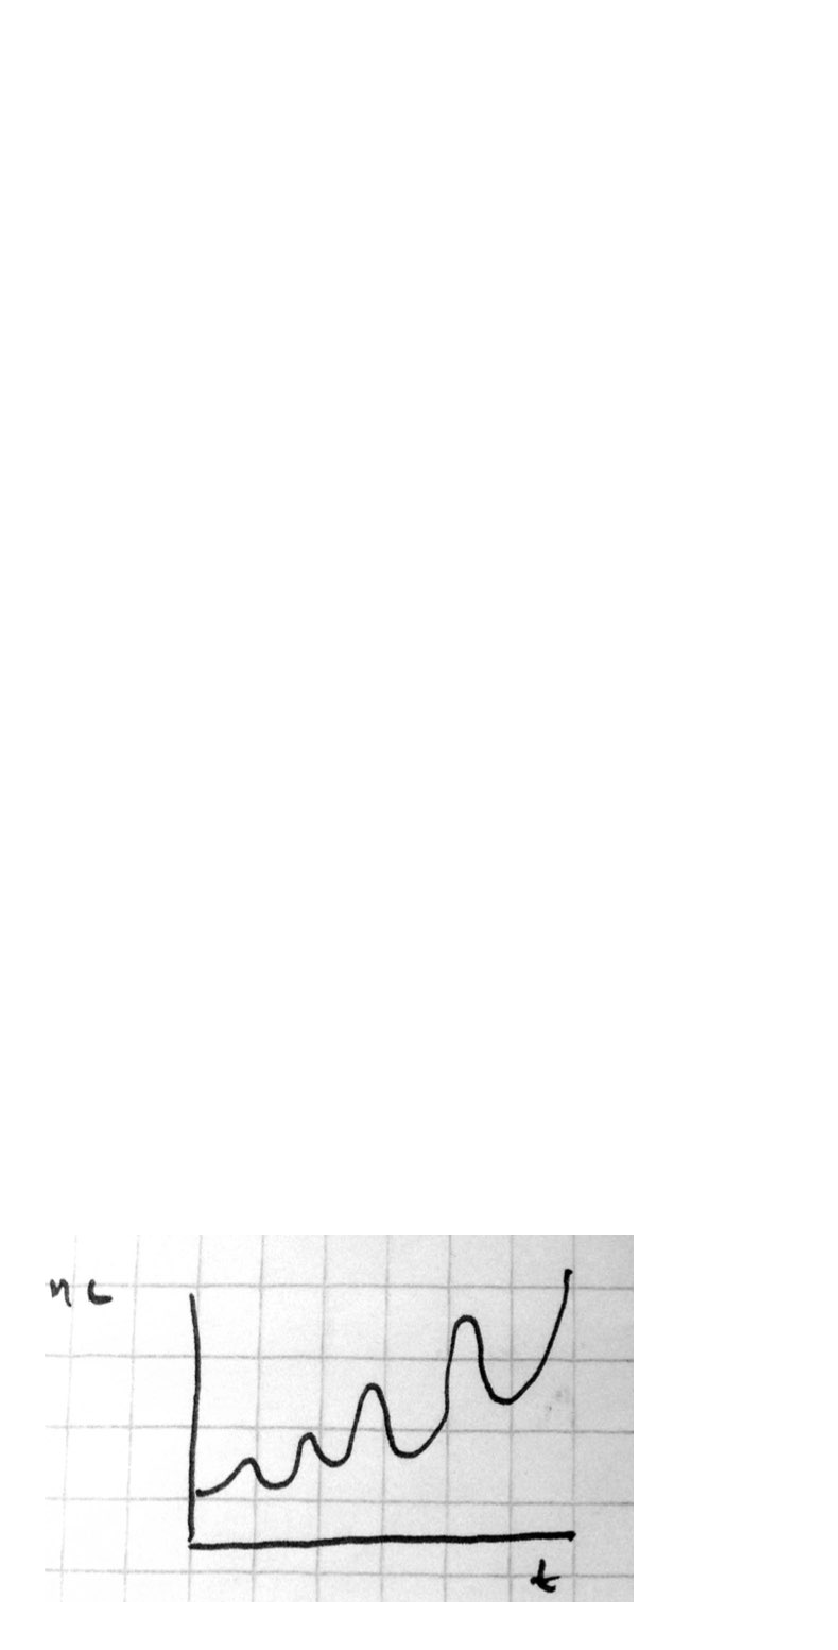
\includegraphics[width=3cm]{figs/GrowthOscil.pdf}
\end{center}

\textbf{For continuous model:}\\
\begin{equation*}
\boxed{	\left.\frac{d\; f(N)}{dN} \right \vert_{N^*}<0  \; \text{for stability}}
\end{equation*}

We'll get much deeper into stability of continuous-time models from now on.  \\
Will also talk about how oscillations occur and how their presence is analytically determined. 

\vspace{1cm}
\textbf{Remember} that we're only dealing with \textbf{local} stability (i.e. small $n_t$) not global stability!
\begin{center}
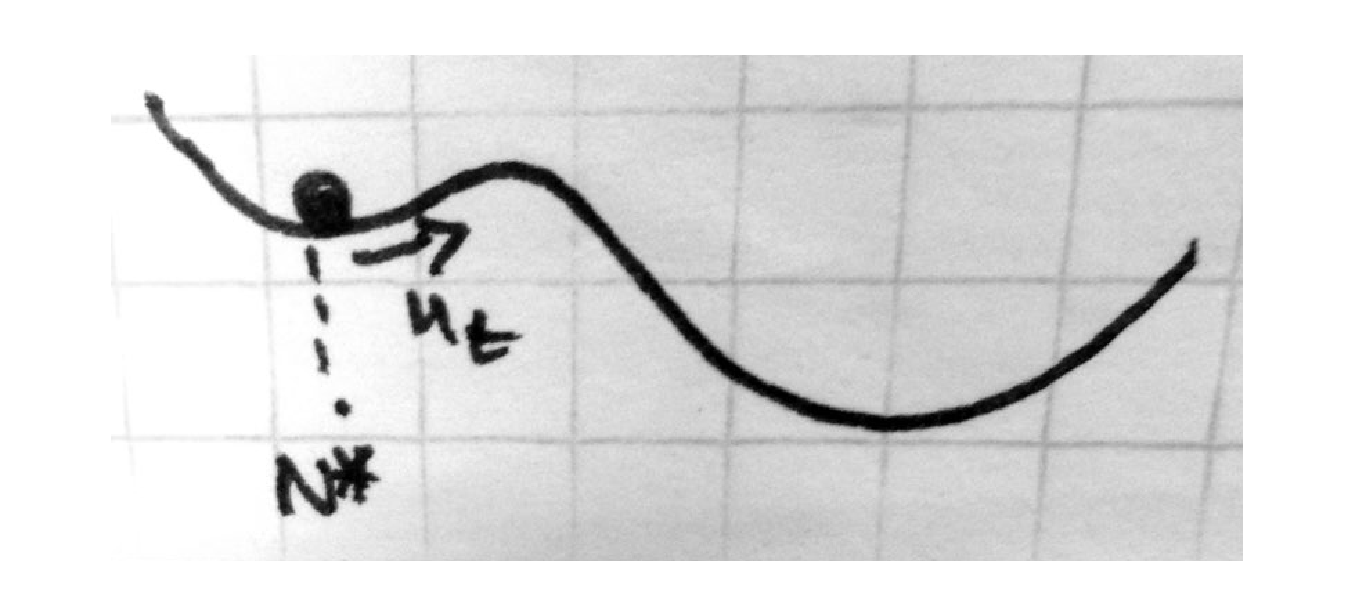
\includegraphics[width=6cm]{figs/LocalStability.pdf}
\end{center}

\rule[0.5ex]{\linewidth}{1pt}

\textbf{Intro to Mathematica}\\
\ind \textbf{Local stability analysis of continuous logistic}

\begin{center}
\note{Walk through Mathematica code: \emph{'Class9-Stability-cLogistic.nb'}}
\end{center}

Functions use square brackets [ ].

Important functions:\\
\ind \emph{Solve[y=ax,x]}\\
\ind \emph{D[f(x),x]}\\
\ind \emph{Simplify}\\
\ind $func\; /. \; x \to y$\\ 
\ind $var\; /. \; x$\\


\rule[0.5ex]{\linewidth}{1pt}

\pagebreak

\textbf{Non-dimensionalization}\\
The equation
\begin{equation*}
	\frac{dN}{dt}=rN\left(1-\frac{N}{K}\right) = \lim_{\Delta t\to 0}\left(\frac{\Delta N}{\Delta t}\right)
\end{equation*}
has 2 parameters (+1 that's implicit!) and 1 variable.\\
\ind \ind $r : \frac{\#}{\# time}$
\ind \ind $K : \#$
\ind \ind $N : \#$

\vspace{1cm}

Define $x$ to be the population size relative to the carrying capacity (i.e. fraction of the carrying capacity).:
\begin{equation*}
	x := \frac{N}{K}
\end{equation*}

$x$ is dimensionless!

\vspace{0.5cm}

(Note:  The symbol $:=$ means \emph{define}.  Sometimes the symbol $\equiv$ meaning \emph{equivalent} is also used.)

\vspace{0.5cm}

Rearrange to $N=xK$ and substitute:
\begin{align*}
      \frac{dxK}{dt}&=rxK \left( 1- \frac{xK}{K} \right)\\
       \frac{dx}{dt}&=rx \left( 1- x \right)
\end{align*}

Only 1 variable ($x$ )and 1 parameter ($r$), same dynamical properties.

Can reduce further...

\begin{equation*}
	\tau := r t
\end{equation*}
($\tau$ = `tau') - dimensionless - the units of $r$ are \#'s per \# per time $(=1/t)$. 

That is,
\begin{equation*} 
	\frac{d}{dt} = \frac{d}{d\tau} \cdot \frac{d\tau}{dt} 
\end{equation*}
Rewriting $r=\tau/t =d\tau/dt  $, this simplifies to
\begin{equation*}
	\frac{d}{dt} = \frac{d}{d\tau}r
\end{equation*}

\vspace{0.5cm}
Therefore
\begin{align*}
       \frac{dx}{dt}&=rx \left( 1- x \right)\\
       \frac{drx}{d\tau}&=rx \left( 1- x \right)\\
       \frac{dx}{d\tau}&=x \left( 1- x \right)
\end{align*}

Only 1 variable and 0 parameters!!!


Of course, `time-scale' $\tau$ is tricky to conceptualize.\\
\ind $\to$ scaled realized rate of population dynamics (i.e. $dN/dt$ or $dx/dt$)...\\
\ind \ind ...relative to the maximum growth rate of the population ($r$). \\

Model is thus in terms of the realized growth relative to the maximum intrinsic growth.\\

Won't do all that much more non-dimensionalization (except in 2-spp. competition model, next), but can be extremely useful.\\
e.g., when absolute values of parameters are not known, but their relative values is (or can be approximated, or qualitatively known  $>1$ or $< 1$)


\end{document}